\documentclass[]{scrartcl}
\usepackage{graphicx}
\usepackage{color}
\usepackage{hyperref}
\usepackage{calc} 
\usepackage{enumitem}
\newcommand{\source}[1]{\vspace{-3pt} \caption*{ Source: {#1}} }
%\pagestyle{headings}

% customize dictum format:
\usepackage[T1]{fontenc}
\setkomafont{dictumtext}{\itshape\small}
\setkomafont{dictumauthor}{\normalfont}
\renewcommand*\dictumwidth{\linewidth}
\renewcommand*\dictumauthorformat[1]{--- #1}
\renewcommand*\dictumrule{}
\newcommand{\todo}[1]{\textcolor{red}{TODO: #1}\PackageWarning{TODO:}{#1!}}

\begin{document}

\title{
	\includegraphics*[width=0.63\textwidth]{images/yale_logo.png}\\
	\vspace{24pt}
	ENGL 300:\\Introduction to Theory of Literature}
\subtitle{Lecture Spring, 2009\\
          Paul H. Fry\\
          William Lampson Professor of English \\ 
          Yale University}
\author{Lennard Wolf\\
        \href{mailto:lennard.wolf@student.hu-berlin.de}{lennard.wolf@student.hu-berlin.de}}
\maketitle
\begin{abstract}

This is a survey of the main trends in twentieth-century literary theory. Lectures will provide background for the readings and explicate them where appropriate, while attempting to develop a coherent overall context that incorporates philosophical and social perspectives on the recurrent questions: what is literature, how is it produced, how can it be understood, and what is its purpose?

\end{abstract}
\newpage

\tableofcontents

\listoffigures
\newpage


\section{Introduction I}

\dictum[William Wordsworth, \textit{The Friend, 1805}]{%
Bliss was it in that dawn to be alive}


\subsection{Description Text}
In this first lecture, Professor Paul Fry explores the course's title in three parts. The relationship between theory and philosophy, the question of what literature is and does, and what constitutes an introduction are interrogated. The professor then situates the emergence of literary theory in the history of modern criticism and, through an analysis of major thinkers such as Marx, Nietzsche, and Freud, provides antecedents for twentieth-century theoretical developments.

\subsection{Content}

Literature can not really be defined clearly, as exceptions to the rule always persist. However defining it helps us deal with complexity, and to understand what literature is, is in part goal of this lecture. \emph{Theory} has the goal of analyzing the text to for example understand its meaning and can thus be put to practice using certain methodologies. Questions raised by Literary Theory can be \emph{"What is a reader/an author?"} etc.

Scepticism has its roots in \emph{Modernity}

Modern criticism has three central figures: Marx, Nietzsche, and Freud.  

\subsection{New Words}

\begin{description}[leftmargin=!,labelwidth=\widthof{\bfseries Literary Theory}]
  \item[Literature] Literature can not really be defined clearly, as exceptions to the rule always persist. Thus definitions of literature can always only exist in a certain context.
  \item[Hermeneutics] The science of interpreting and understanding of human symbols, usually in the form of text.
  \item[Literary Theory] In contrast to \emph{Literary Criticism}, Literary Theory is not concerned with opinionating and finding the value of the text, but rather with systematically analyzing and dwelling on the text while considering history, philosophy, and other fields which are relevant to the interpretation of meaning. Today, it is often referred to as \emph{Theory} in the academic world.
  \item[Modernity] (Not to be confused with \emph{Modernism}) ??
  \item[Cartesian Revolution] ??
\end{description}

\section{Introduction II}

%\textcolor{red}{Fehlendes Bild}

\textcolor{red}{Fehlender Text}


\newpage
\section{Meta}
\subsection{The Professor}
Prof. Paul H. Fry (see Figure \ref{fig:paul_fry}) received his B.A. from University of California, Berkeley in 1966 and earned his Ph.D. in 1973 from Harvard University, where he had writ7ten his dissertation \emph{"Byron’s Myth of the Self"}. He has taught at Yale University since 1971, became Assistant Professor of English in 1973, Associate Professor of English in 1979, Professor of English in 1985 and William Lampson Professor of English in 1993.

\begin{figure}[]
	\centering
	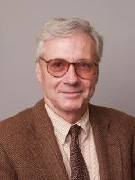
\includegraphics[width=0.32\textwidth]{images/paul_fry.jpg}
	\caption{Prof. Paul Fry. Source: \url{https://www.library.yale.edu/judaica/site/conferences/Amichai/Speaker\%20pics/roundtable/Fry_1051.jpg}}
	\label{fig:paul_fry}
\end{figure}

\subsection{Texts}

Richter, David, ed. The Critical Tradition, 3rd ed. (Bedford-St. Martin's, 2006)


\end{document}
